\documentclass[10pt,a4paper]{article}
\usepackage[margin=21mm,headheight=15pt]{geometry}
\usepackage[T1]{fontenc}
\usepackage{lmodern,amsmath,amssymb,tikz,graphicx,hyperref,fancyhdr,enumitem}
\usetikzlibrary{arrows.meta,positioning,calc,decorations.pathmorphing}
\definecolor{ink}{RGB}{20,53,78}
\hypersetup{colorlinks=true,urlcolor=ink,linkcolor=ink}
\setlength{\parindent}{0pt}\setlength{\parskip}{5pt}
\emergencystretch=3em
\pagestyle{fancy}\fancyhf{}\fancyfoot[C]{\thepage}
\renewcommand{\headrulewidth}{.3pt}
\newcommand{\task}[2]{\par\medskip{\color{ink}\Large\bfseries #1. #2}\par\smallskip}
\newcommand{\answer}{\par\smallskip\textbf{Worked reasoning.} }
\setlist[enumerate]{label=\textbf{(\alph*)},leftmargin=7mm,itemsep=7pt}
\begin{document}
\fancyhead[L]{\small Control of Dynamical Systems}
\fancyhead[R]{\small Laboratory 03}
{\color{ink}\LARGE\bfseries Laboratory 03}\par
{\large A precision platform under floor motion}\par
\textbf{Worked solutions -- five integrated problems}\par
{\small\textbf{Evidence boundary.} Original hypothetical scenarios. Derive, calculate and justify decisions; every numerical record is synthetic. Figures are conceptual and not to scale.}
\smallskip\textbf{Shared nominal data.} Nominal payload: $m=8$ kg, $k=3200$ N/m and $\zeta=0.08$ unless varied. Absolute payload motion is $x$; floor motion is $z$. Spring and damper depend on relative motion about static equilibrium.
\task{1}{An optical platform on a moving foundation}
A precision payload is supported by a spring and damper attached to a moving floor. Positions are measured about the loaded static equilibrium, so gravity does not appear in the incremental motion equation.
\begin{center}\resizebox{.80\linewidth}{!}{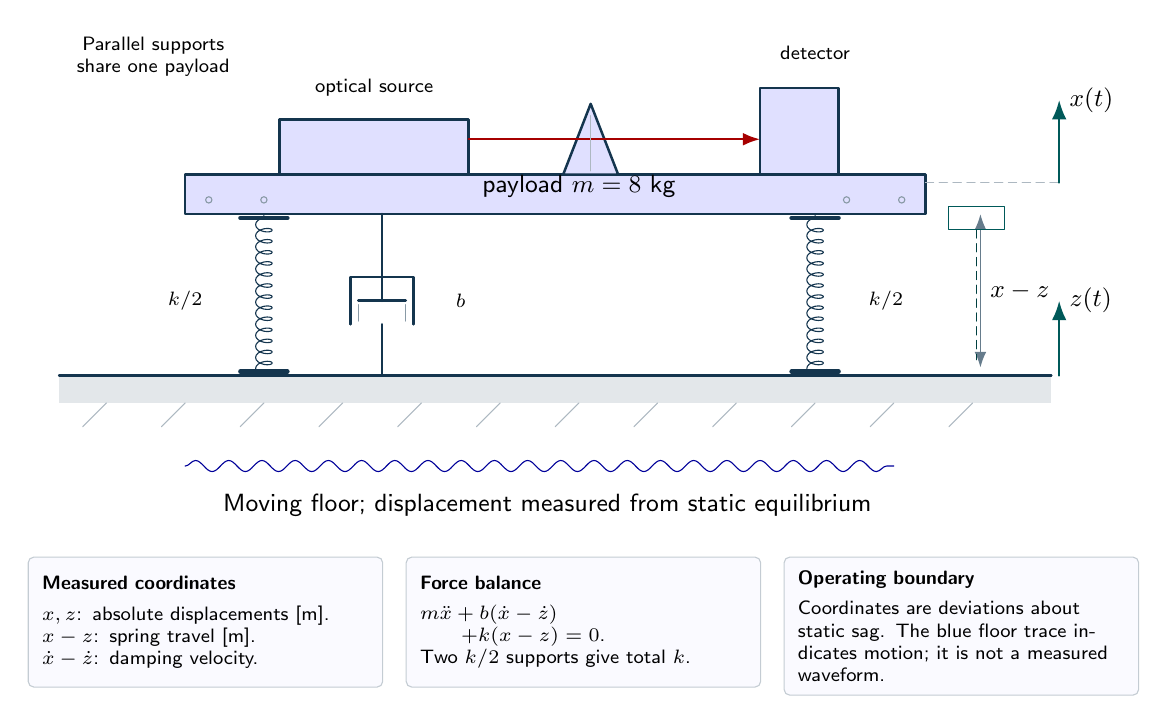
\begin{tikzpicture}[
font=\sffamily\small,>=Latex,line cap=round,line join=round,
wall/.style={draw=ink,line width=1.2pt,fill=blue!5},
water/.style={fill=cyan!25,draw=none},
metal/.style={draw=ink,fill=blue!12,line width=.9pt},
flow/.style={->,draw=blue!65!black,line width=1.2pt},
heat/.style={->,draw=orange!85!black,line width=1.1pt},
measure/.style={->,draw=teal!70!black,line width=.9pt},
dim/.style={<->,draw=ink!65,line width=.6pt},
spring/.style={draw=ink,decorate,decoration={coil,aspect=.5,segment length=4pt,amplitude=3pt}},
wire/.style={draw=ink,line width=1pt},
lab/.style={align=center,font=\sffamily\small},
smalllab/.style={align=center,font=\sffamily\scriptsize}]

\fill[ink!12](.4,.2)rectangle(13,.55);
\draw[ink,line width=1pt](.4,.55)--(13,.55);
\foreach \x in {1,2,...,12}{\draw[ink!35](\x,.2)--++(-.3,-.3);}
\draw[metal](2,2.6)rectangle(11.4,3.1);
\draw[spring](3,.55)--(3,2.6);
\draw[spring](10,.55)--(10,2.6);
\draw[wire](4.5,.55)--(4.5,1.2)(4.1,1.2)--(4.1,1.8)--(4.9,1.8)--(4.9,1.2);
\draw[wire](4.5,2.6)--(4.5,1.5)(4.2,1.5)--(4.8,1.5);
\draw[metal](3.2,3.1)rectangle(5.6,3.8);
\draw[metal](6.8,3.1)--(7.15,4)--(7.5,3.1)--cycle;
\draw[metal](9.3,3.1)rectangle(10.3,4.2);
\draw[red!65!black,->,line width=.7pt](5.6,3.55)--(9.3,3.55);
\node[smalllab]at(4.4,4.2){optical source};
\node[smalllab]at(10,4.65){detector};
\node[lab]at(7,2.95){payload $m=8$ kg};
\node[smalllab]at(2,1.5){$k/2$};\node[smalllab]at(10.9,1.5){$k/2$};
\node[smalllab]at(5.5,1.5){$b$};
\draw[dim](12.1,.65)--node[right]{$x-z$}(12.1,2.6);
\draw[ink!35,densely dashed](11.4,3)--(13.1,3);
\draw[measure](13.1,3)--(13.1,4.05)node[right]{$x(t)$};
\draw[measure](13.1,.55)--(13.1,1.5)node[right]{$z(t)$};
\draw[blue!60!black,decorate,decoration={snake,amplitude=2pt,segment length=12pt}](2,-.6)--(11,-.6);
\node[lab]at(6.6,-1.1){Moving floor; displacement measured from static equilibrium};
% REFINED EQUIPMENT DETAILS

% Fasteners, spring seats and a clearly resolved dashpot piston.
\foreach \x in {2.3,3,10.4,11.1}{\draw[ink!50](\x,2.78)circle(.04);}
\foreach \x in {3,10}{\draw[ink,line width=1.5pt](\x-.3,.6)--(\x+.3,.6)(\x-.3,2.55)--(\x+.3,2.55);}
\draw[ink!50](4.2,1.24)--(4.2,1.45)(4.8,1.24)--(4.8,1.45);
\draw[ink!35](7.15,3.15)--(7.15,3.85);
\draw[teal!70!black](11.7,2.4)rectangle(12.4,2.7);
\draw[teal!50!black,densely dashed](12.05,2.4)--(12.05,.75);
\node[smalllab,anchor=west]at(.5,4.6){Parallel supports\\share one payload};

\node[draw=ink!25,fill=blue!2,rounded corners=2pt,anchor=north west,text width=4.15cm,minimum height=1.65cm,inner sep=5pt,align=left,font=\sffamily\scriptsize]at(0.0,-1.75){\textbf{Measured coordinates}\\[3pt]$x,z$: absolute displacements [m].\\$x-z$: spring travel [m].\\$\dot x-\dot z$: damping velocity.};
\node[draw=ink!25,fill=blue!2,rounded corners=2pt,anchor=north west,text width=4.15cm,minimum height=1.65cm,inner sep=5pt,align=left,font=\sffamily\scriptsize]at(4.8,-1.75){\textbf{Force balance}\\[3pt]$m\ddot x+b(\dot x-\dot z)$\\$\qquad+k(x-z)=0$.\\Two $k/2$ supports give total $k$.};
\node[draw=ink!25,fill=blue!2,rounded corners=2pt,anchor=north west,text width=4.15cm,minimum height=1.65cm,inner sep=5pt,align=left,font=\sffamily\scriptsize]at(9.6,-1.75){\textbf{Operating boundary}\\[3pt]Coordinates are deviations about static sag. The blue floor trace indicates motion; it is not a measured waveform.};
\end{tikzpicture}
}\par{\small An optical payload rests on parallel spring and damping elements. The two springs each have stiffness $k/2$, giving total $k$. Both the floor and payload move; spring extension and damping velocity are relative quantities. Weight is balanced at the static equilibrium about which the model is written.}\end{center}
\begin{enumerate}
\item An 8 kg platform is attached to a moving floor by a spring $k=3200$ N/m and damper $b$. Let $x$ and $z$ be absolute platform and floor displacements. Derive $X/Z$ and the relative-displacement transfer $(X-Z)/Z$.
\answer Forces depend on relative deformation and velocity: $m\ddot x=-b(\dot x-\dot z)-k(x-z)$. Therefore $X/Z=(bs+k)/(ms^2+bs+k)$. Subtracting one gives $(X-Z)/Z=-ms^2/(ms^2+bs+k)$. Replacing the moving floor by an applied force would change the numerator and the isolation interpretation; the two input models are not interchangeable.
\item Find $\omega_n$ and the damping coefficients for ratios 0.08 and 0.4. Calculate the closed-form poles for both cases.
\answer The natural frequency is $\sqrt{k/m}=20$ rad/s. From $b=2\zeta\sqrt{mk}=320\zeta$, the damping coefficients are 25.6 and 128 N s/m. The poles are $-\zeta\omega_n\pm j\omega_n\sqrt{1-\zeta^2}$: $-1.6\pm j\,20\sqrt{0.9936}$ and $-8\pm j\,20\sqrt{0.84}$. Both are stable underdamped pairs. Increasing damping moves the real parts left while reducing damped frequency.
\item Find the zero-frequency gains from floor displacement to absolute payload motion and to relative suspension travel. Explain the physical difference and why using the force-input transfer for this experiment would be wrong.
\answer With $G_{xz}=(bs+k)/(ms^2+bs+k)$, $G_{xz}(0)=1$. Relative travel has $G_{(x-z)z}=G_{xz}-1=-ms^2/(ms^2+bs+k)$, giving zero DC gain. A sufficiently slow floor displacement moves the entire payload without incremental suspension deflection. A separately applied force instead uses $G_{xf}=1/(ms^2+bs+k)$, with different units and numerator; floor displacement is not a force.
\end{enumerate}

\newpage
\task{2}{Damping a resonance while preserving isolation}
The design must cross a resonant region during operation but should isolate higher-frequency floor motion. Compare the competing effects of damping rather than ranking one damper as universally better.
\begin{enumerate}
\item Using $r=\omega/\omega_n$, derive the condition for absolute displacement transmissibility below one. Explain why the nonzero threshold is independent of positive damping in this ideal model.
\answer The squared transmissibility is $T^2=[1+(2\zeta r)^2]/[(1-r^2)^2+(2\zeta r)^2]$. For $T^2<1$, subtract the common damping terms: $1<(1-r^2)^2$, or $r^2(r^2-2)>0$. Hence isolation begins at $r>\sqrt2$, namely $\omega>20\sqrt2\approx28.284$ rad/s. At $r=0$ and $r=\sqrt2$, $T=1$. The cancellation follows from this specific base-excitation numerator.
\item Calculate transmissibility at $r=1$ for damping ratios 0.08 and 0.4. Which design better suppresses floor motion at that frequency? Do these values necessarily equal the exact peak magnitudes?
\answer At $r=1$, $T=\sqrt{1+4\zeta^2}/(2\zeta)$. The two values are $\sqrt{1.0256}/0.16\approx6.3295$ and $\sqrt{1.64}/0.8\approx1.6008$. The larger damping transmits less motion at this frequency. The base-excited transfer has a zero, so its exact magnitude maximum need not occur at $\omega_n$. Evaluating at $r=1$ is a useful comparison, not a proof of the peak frequency.
\item Analyze the limit $\zeta\to0^+$ at $r=1$ and at a fixed $r>\sqrt2$. Use the result to explain why an isolation threshold alone is an incomplete design specification.
\answer At $r=1$, the transmissibility is $\sqrt{1+4\zeta^2}/(2\zeta)$ and diverges as damping tends to zero. At fixed $r>\sqrt2$, its limit is $1/(r^2-1)<1$. Thus a weakly damped system can isolate well above resonance while suffering an arbitrarily large resonant amplification. The threshold $r=\sqrt2$ does not constrain the peak, decay time, usable travel or force limits.
\end{enumerate}

\newpage
\task{3}{Absolute vibration and suspension-travel limits}
The same floor motion can create different specifications for the optical payload and its supporting suspension. Evaluate both outputs before selecting a mount.
\begin{center}\resizebox{\ifdim\width>.98\linewidth.98\linewidth\else\width\fi}{!}{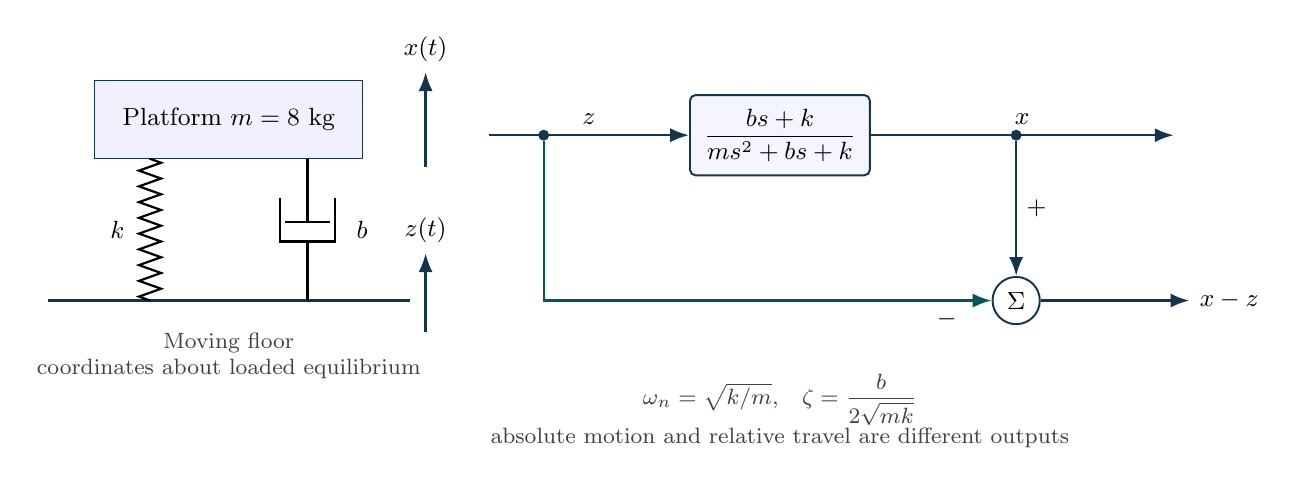
\begin{tikzpicture}[x=1cm,y=1cm,>=Latex,font=\small,
block/.style={draw=ink,fill=blue!4,rounded corners=2pt,minimum height=9mm,align=center,line width=.7pt,inner sep=5pt},
sum/.style={circle,draw=ink,fill=white,minimum size=6mm,inner sep=0pt,line width=.7pt},
sig/.style={->,draw=ink,line width=.85pt},
fb/.style={->,draw=teal!70!black,line width=.85pt},
dist/.style={->,draw=orange!75!black,line width=.85pt},
tap/.style={circle,fill=ink,inner sep=1.4pt},
note/.style={font=\footnotesize,align=center,text=black!75}]

\node[draw=ink,fill=blue!6,minimum width=34mm,minimum height=10mm](m)at(2,2.2){Platform $m=8$ kg};
\draw[line width=1.2pt,draw=ink](-.3,-.1)--(4.3,-.1);
\draw[decorate,decoration={zigzag,segment length=2mm,amplitude=1.4mm},line width=.8pt](1,-.1)--(1,1.7);
\node[left]at(.8,.8){$k$};
\draw[line width=.8pt](3,-.1)--(3,.65);
\draw[line width=.8pt](2.65,1.2)--(2.65,.65)--(3.35,.65)--(3.35,1.2);
\draw[line width=.8pt](2.72,.9)--(3.28,.9);
\draw[line width=.8pt](3,.9)--(3,1.7);
\node[right]at(3.5,.8){$b$};
\draw[sig](4.5,1.6)--(4.5,2.8)node[above]{$x(t)$};
\draw[sig](4.5,-.5)--(4.5,.5)node[above]{$z(t)$};
\node[note]at(2,-.8){Moving floor\\coordinates about loaded equilibrium};
\node[block](g)at(9,2){$\dfrac{bs+k}{ms^2+bs+k}$};
\node[tap](zt)at(6,2){};
\node[tap](xt)at(12,2){};
\draw[sig](5.3,2)--node[above]{$z$}(g);
\draw[sig](g)--node[above]{$x$}(14,2);
\node[sum](rel)at(12,-.1){$\Sigma$};
\draw[sig](xt)--node[right]{$+$}(rel);
\draw[fb](zt)--(6,-.1)--node[pos=.9,below]{$-$}(rel);
\draw[sig](rel)--(14.2,-.1)node[right]{$x-z$};
\node[note]at(9,-1.5){$\omega_n=\sqrt{k/m}$,\quad $\zeta=\dfrac{b}{2\sqrt{mk}}$\\absolute motion and relative travel are different outputs};

\end{tikzpicture}
}\par{\small Base excitation drives absolute motion; subtracting the floor coordinate gives relative travel. The spring and damper act in parallel.}\end{center}
\begin{enumerate}
\item Evaluate transmissibility at $r=3$ for both damping ratios. For nonzero damping, derive the high-frequency asymptote and explain the design conflict with Problem 2(b).
\answer Substitution gives $T_{0.08}=\sqrt{1.2304/64.2304}\approx0.13841$ and $T_{0.4}=\sqrt{6.76/69.76}\approx0.31130$. At large $r$ and fixed $\zeta>0$, the leading terms give $T\sim2\zeta/r$. Lower damping therefore improves sufficiently high-frequency isolation, even though it increases near-resonance amplification. For exactly zero damping the asymptote is instead $1/r^2$, so the zero-damping limit needs separate treatment.
\item At $r=2$, floor displacement amplitude is 0.5 mm. With $\zeta=0.08$, find the amplitude of relative travel $x-z$ and decide whether it stays within a 0.8 mm amplitude limit.
\answer The relative transfer magnitude is $r^2/\sqrt{(1-r^2)^2+(2\zeta r)^2}$. At $r=2$ it is $4/\sqrt{9+0.1024}\approx1.32581$. Multiplying by 0.5 mm gives approximately 0.66291 mm, below 0.8 mm. This is a steady sinusoidal amplitude test; it does not bound startup transients or arbitrary broadband floor motion.
\item For a fixed floor-displacement amplitude of 0.5 mm, find the limiting absolute and relative amplitudes as frequency tends to infinity with nonzero damping. Relate these limits to the finite-frequency travel check.
\answer As $\omega\to\infty$, $X/Z\sim b/(jm\omega)\to0$, but $(X-Z)/Z\to-1$. The absolute payload amplitude tends to zero while relative travel tends to 0.5 mm, with opposite phase to the floor. At $r=2$ the nominal relative amplitude is about 0.66291 mm, so the asymptotic limit alone would underestimate the travel needed at that operating frequency.
\end{enumerate}

\newpage
\task{4}{A heavier payload under a tight static-sag requirement}
The payload may change, but static support and vibration isolation must still be achieved by the same spring. Treat these as simultaneous constraints.
\begin{enumerate}
\item Keep $k=3200$ and $b=25.6$ but increase total mass to 12 kg. Find the new natural frequency, damping ratio and isolation threshold. Explain why keeping the damper fixed does not keep the damping ratio fixed.
\answer The new frequency is $\omega_n=\sqrt{3200/12}\approx16.3299$ rad/s. The ratio is $\zeta=b/[2\sqrt{mk}]=25.6/[2\sqrt{38400}]\approx0.06532$. The isolation threshold becomes $\sqrt2\omega_n\approx23.0940$ rad/s. Damping ratio is a normalized quantity depending on both mass and stiffness; a fixed physical damper produces a smaller ratio as mass increases.
\item For the original 8 kg platform, calculate static spring deflection under gravity. If deflection may not exceed 3 mm, determine the minimum stiffness and the corresponding natural frequency, using $g=9.81$ m/s$^2$.
\answer The original deflection is $mg/k=8(9.81)/3200=0.024525$ m, or 24.525 mm. The new requirement gives $k\ge mg/0.003=26160$ N/m. At equality, $\omega_n=\sqrt{26160/8}=\sqrt{3270}\approx57.1839$ rad/s. A stiffer support meets static-travel requirements but raises the isolation threshold. The vibration model is understood around the gravity-loaded equilibrium.
\item Require gravity sag at most 3 mm and isolation of floor motion at 40 rad/s. Derive mass-independent bounds on $\omega_n$ and decide whether any passive spring in this model satisfies both.
\answer Static sag is $mg/k=g/\omega_n^2$. The sag requirement gives $\omega_n\ge\sqrt{9.81/0.003}\simeq57.184$ rad/s. Isolation at 40 rad/s requires $40/\omega_n>\sqrt2$, or $\omega_n<28.284$ rad/s. There is no intersection, regardless of payload mass. A different architecture, preload/load-support arrangement or active solution is required; changing the mass without changing the specification cannot remove this conflict.
\end{enumerate}

\newpage
\task{5}{What a decay test says about energy and excitation}
A synthetic ring-down is used to infer damping. Distinguish that unforced test from operation on a moving floor, which can continually inject energy.
\begin{enumerate}
\item In a noise-free synthetic free decay, consecutive positive peaks are 1.5 mm and 0.9 mm, separated by 0.32 s. Infer damping ratio, natural frequency and $b$ if mass is 8 kg. State the assumption behind this inference.
\answer Let $\delta=\ln(1.5/0.9)=\ln(5/3)$. Then $\zeta=\delta/\sqrt{4\pi^2+\delta^2}\approx0.08103$, $\omega_d=2\pi/0.32$, and $\omega_n=\omega_d/\sqrt{1-\zeta^2}\approx19.6997$ rad/s. Finally $b=2m\zeta\omega_n=16\delta/0.32\approx25.5413$ N s/m. The formula assumes one underdamped linear mode, zero continuing excitation, and peaks one complete cycle apart.
\item Set $z=0$. Show that mechanical energy decreases for $b>0$ and discuss asymptotic stability. Explain why the same autonomous energy argument cannot prove decreasing platform energy for arbitrary moving-floor excitation.
\answer Use $E=\tfrac12m\dot x^2+\tfrac12kx^2$. Differentiating and substituting $m\ddot x+b\dot x+kx=0$ gives $\dot E=-b\dot x^2\le0$. The only invariant motion within $\dot x=0$ has $kx=0$, hence $x=0$; with $m,k,b>0$ the origin is asymptotically stable. A moving floor supplies external work through spring and damper forces, so it can inject energy. The unforced proof cannot bound a forced response without accounting for that input.
\item For moving floor coordinate $z$, use physical stored energy $E=m\dot x^2/2+k(x-z)^2/2$. Derive its power balance and identify the term that prevents an unconditional monotonic-decay claim.
\answer Differentiation and $m\ddot x=-b(\dot x-\dot z)-k(x-z)$ give $\dot E=-b(\dot x-\dot z)^2-[b(\dot x-\dot z)+k(x-z)]\dot z$. The first term is nonpositive viscous dissipation. The second is power transferred through the moving support and can have either sign. Setting $\dot z=0$ recovers passive decay, but a ring-down argument cannot bound the response to arbitrary sustained floor motion.
\end{enumerate}

\end{document}
